\documentclass[12pt]{article}
\usepackage[a4paper, margin=0.7in]{geometry}
\usepackage{color}   %May be necessary if you want to color links
\usepackage{hyperref}
\usepackage{graphicx}
\usepackage[paper=portrait,pagesize]{typearea}
\usepackage{minted}
\usemintedstyle{vs}
\usepackage{hhline}
\setlength{\tabcolsep}{18pt}
\renewcommand{\arraystretch}{1.5}
\renewcommand{\contentsname}{Indice}
\begin{document}
\title{Esercitazione Pasqua 2022}
\date{}
\author{Leonardo Geusa 4N}
\setcounter{section}{-1}
\maketitle

Un ospedale vuole innovare la sua infrastruttura tecnologica per realizzare servizi interni. L’ospedale è
composto da 4 reparti distribuiti su due piani(ogni reparto si sviluppa su un unico piano). Ogni medico di
reparto, dopo avere visitato un paziente, può collegarsi in modalità wireless ad un server web interno,
dislocato in un locale tecnico posto al piano seminterrato, per registrare le informazioni medico-sanitarie
dei pazienti visitati oppure visualizzare la scheda del paziente. Nel locale tecnico è presente oltre al server
web anche un server DHCP per l’assegnazione automatica degli indirizzi IP ai vari dispositivi e un server
DNS. In ogni reparto è presente anche una saletta medica con due postazioni fisse e una stampante.
Al piano seminterrato è presente anche la farmacia composta da due postazioni fisse e una stampante.
In riferimento anche allo standard di cablaggio IEC 11801, realizzare la documentazione di rete (minisito o
word) indicando:
\begin{itemize}
	\item La topologia fisica applicata.
	\item I dispositivi utilizzati e le loro caratteristiche tecniche
	\item I mezzi di trasmissione utilizzati sia per il cablaggio verticale che orizzontale e le loro caratteristiche tecniche.
	\item Il tipo di connessione ad internet adottata e le sue caratteristiche. Il tipo di connessione deve essere scelta tra quelle viste (ADSL, FTTC, FTTB, FTTH) che meglio si adatta allo scenario.
	\item Il piano di indirizzamento
	\item Disegno di rete indicando una configurazione dell’access point, dei server e dei pc.
	\item Inoltre l’ospedale si vuole estendere aprendo una rete di ambulatori sul territorio cittadino. Ciascun ambulatorio sarà costituito da un ufficio amministrativo (1 pc e una stampante) e da una sala per la visita del paziente (1 pc). Ciascun ambulatorio deve interfacciarsi con la sede centrale. Per realizzare il disegno su packet tracer considerare due ambulatori collegati al router dell’ospedale mediante linea seriale. Indicare la tabella di instradamento dei tre router.
\end{itemize}

Facendo riferimento alla struttura del solo ospedale e volendo realizzare per ogni reparto inclusa la
farmacia una vlan e che solo la farmacia possa collegarsi ad internet, come cambia la struttura della rete?
Indicare la diversa configurazione.
\newpage
\vspace*{3cm}
\tableofcontents



\raggedright

\section{Ipotesi aggiuntive}
\hspace{24pt}
Si presuppone che l'ospedale abbia intenzione di investire tanto capitale in modo tale da rendere
la rete il più efficiente e moderna possibile.

\section{Analisi della struttura e delle esigenze degli edifici}

Secondo le informazioni ricevute, l'intervento avverrà in 6 locali dell'ospedale disposti su tre piani:
\begin{itemize}
	\item al piano terra due reparti
	\item al primo piano due reparti
	\item al piano seminterrato una sala server e una farmacia
\end{itemize}
Un reparto è costituito da un totale di 3 postazioni e una stampante.\\
La sala server ha al suo interno 3 server (uno per il servizio web, uno per il DHCP e uno per il DNS).\\
La farmacia è composta da 2 postazioni e una stampante.\\
Saranno presenti anche due ambulatori nella città, ognuno con un totale di due postazioni e una stampante. \\
Sono necessari quindi 3 server, 18 postazioni e 7 stampanti di rete.
La rete deve essere efficiente e scalabile, perciò si ha bisogno di cavi e nodi di commutazione che possano soddisfare al massimo queste due richieste.

\section{Analisi della topologia fisica e logica}
\hspace{24pt}Per questo progetto si realizzerà una MAN, composta da diverse LAN (e WLAN) a stella estesa collegate tra 
di loro tramite dei router. \\
\hspace{24pt}La topologia logica che si andrà ad applicare sarà di tipo broadcast, ossia ogni nodo invia i dati 
mediante una scheda di rete a tutti gli altri nodi. Nell'ipotesi della VLAN, però, anche se connessi alla stessa rete 
fisica, due dispositivi appartenenti a due VLAN differenti non potranno comunicare in alcun modo, neanche tramite 
broadcast.

\section{Analisi degli apparati di rete e mezzi trasmissivi}
Per quanto riguarda gli apparati di rete si andranno ad utilizzare schede di rete, router, AP e switch.\\
\hspace{24pt}La scheda di rete è un dispositivo elettronico installato all'interno di un host che permette il collegamento tra l'host e il cavo, che collega i vari nodi. Una scheda di rete può essere wireless, ossia non ha bisogno di un collegamento fisico via cavo, bensì comunica con l'AP tramite onde radio (etere).\\
\hspace{24pt}Il router è un dispositivo che permette la connessione tra due reti, in particolare una rete LAN e Internet. In questo progetto mette in comunicazione la rete della scuola con la rete Internet.\\
\hspace{24pt}Lo switch è un dispositivo che collega insieme altri dispositivi. Lo switch, rispetto all'hub, gestisce in modo più efficiente il trasporto dei dati perché inoltra il pacchetto ricevuto soltanto al destinatario.\\
\hspace{24pt}L'AP è un particolare tipo di switch che permette di collegare dispositivi possedenti una scheda di rete wireless, onde evitare di utilizzare troppi cavi. Un AP può essere pubblico o protetto. Se è pubblico non ha bisogno di una chiave d'accesso, se è protetto allora può utilizzare diversi sistemi di sicurezza. Il sistema WEP\footnote{Wired Equivalent Privacy, parte dello standard IEEE 802.11. Questo sistema di crittografia delle reti Wi-Fi fu introdotto per evitare il furto dei dati wireless da parte degli hacker.} prevede la presenza di una chiave per connettersi all'AP. I dati verranno criptati tramite questa chiave, in modo da renderli leggibili soltanto da chi è in possesso della chiave. Un'altro sistema di crittografia è quello di WPA/WPA2\footnote{Wi-Fi Protected Access}, più moderno e più sicuro del WEP.\\
\hspace{24pt}Per il cablaggio verticale saranno presenti dorsali di edificio che collegheranno il centro stella di edificio con gli switch di piano. Da qui verranno effettuati i collegamenti alle prese utente, che fanno parte del cablaggio orizzontale.

\section{Piano di indirizzamento e tabella di routing}
\hspace{24pt}Si procede alla stesura del piano di indirizzamento.\\
L'ospedale avrà come indirizzo di rete 192.168.0.0/24. L'interfaccia interna del router dell'ospedale (default gateway) avrà come indirizzo IP 192.168.0.1.
A tutti gli host connessi alla rete interna dell'ospedale sarà assegnato un indirizzo IP in modalità dinamica, tramite un
apposito server DHCP locato nella sala server (192.168.0.2), ad eccezione del server web e del server DNS, il cui indirizzamento
sarà statico (rispettivamente 192.168.0.3 e 192.168.0.4).\\
\hspace{24pt}I due ambulatori, che per comodità si chiamano 1 e 2, avranno gli indirizzi di rete 192.168.1.0/24 e 192.168.2.0/24 e
l'indirizzamento sarà statico data la poca quantità di host appartenenti alla rete. Oltre all'indirizzo IP dell'host 
bisognerà specificare anche il default gateway e il server DNS.\\
\hspace{24pt}Il router dell'ospedale è collegato ai router dei due ambulatori tramite interfacce seriali, a cui sono stati assegnati
indirizzi di classe A. Di seguito la tabella di indirizzamento dei router. \\
\vspace*{12pt}
\begin{center}
    \begin{tabular}{| c | c | c |}
        \hline
        Router       & Interfaccia & Indirizzo IP \\ \hline
        Ospedale     & FA0/0       & 192.168.0.1  \\  \hline
        Ospedale     & SE0/0/0     & 20.0.0.1     \\ \hline
        Ospedale     & SE0/0/1     & 10.0.0.1     \\ \hline
        Ambulatorio1 & FA0/0       & 192.168.1.1  \\ \hline
        Ambulatorio1 & SE0/0/0     & 10.0.0.2     \\ \hline
        Ambulatorio2 & FA0/0       & 192.168.2.1  \\ \hline
        Ambulatorio2 & SE0/0/0     & 20.0.0.2     \\ \hline
    \end{tabular}
\end{center}

\vspace{12pt}
Per far comunicare i due ambulatori con l'ospedale bisogna configurare le tabelle di routing dei router. Si assume che
i due ambulatori non debbano comunicare tra di loro. Di seguito le tabelle per ogni router.\\
\vspace{12pt}
Ospedale:
\begin{center}
    \begin{tabular}{| c | c | c |}
        \hline
        Destinazione & Subnet Mask   & Next Hop \\ \hline
        192.168.1.0  & 255.255.255.0 & 10.0.0.2 \\ \hline
        192.168.2.0  & 255.255.255.0 & 20.0.0.2 \\ \hline
    \end{tabular}
\end{center}
\vspace*{12pt}
Ambulatorio1:
\begin{center}
    \begin{tabular}{| c | c | c |}
        \hline
        Destinazione & Subnet Mask   & Next Hop \\ \hline
        192.168.0.0  & 255.255.255.0 & 10.0.0.1 \\ \hline
    \end{tabular}
\end{center}
\vspace*{12pt}
Ambulatorio2:
\begin{center}
    \begin{tabular}{| c | c | c |}
        \hline
        Destinazione & Subnet Mask   & Next Hop \\ \hline
        192.168.0.0  & 255.255.255.0 & 10.0.0.2 \\ \hline
    \end{tabular}
\end{center}
\vspace*{12pt}


\section{Progettazione della rete}
\hspace{24pt}Per la realizzazione di questa rete è necessario che ogni host (postazioni e stampanti) abbiano una scheda 
di rete di 1 GBit/s. Tutti gli host presenti al piano terra e al primo piano devono essere forniti di una scheda 
di rete wireless. Per sfruttare al massimo queste schede di rete è necessario che anche gli switch (di piano e non) 
e gli AP abbiano porte da 1 GBit/s. Si ha infine bisogno dei cavi, in questo caso UTP\footnote{Unshielded Twisted Pair} 
di 1 GBit/s di categoria 6, con connettori RJ-45. Tenendo sempre in considerazione la scalabilità e la flessibilità 
della rete, si ha quindi bisogno dei seguenti dispositivi di rete:\\
\begin{itemize}
	\item 7 switch: uno da 4 porte per la sala server, uno da 8 porte per la farmacia del seminterrato, 
	tre da 4 porte per i centri stella di piano e di edificio, due da 8 porte per gli ambulatori
	\item 3 router, per la connessione tra ospedale e ambulatori
	\item 2 AP, per la connessione wireless del piano terra e del primo piano
	\item 15 cavi UTP: 12 per le connessioni host - switch, 3 per le connessioni centro stella 
		  di edificio/piano - router 
\end{itemize}
Supponendo che la direzione dell'ospedale abbia bisogno di una rete veloce e che non abbia "limiti" di budget, i 
collegamenti tra i centri stella di piano e le prese utente, e tra i centri stella di piano e il centro stella di 
edificio saranno realizzati in fibra ottica (FTTH).
Di seguito la rappresentazione grafica della rete.
\vspace*{24pt}
\begin{center}
	\makebox[\textwidth]{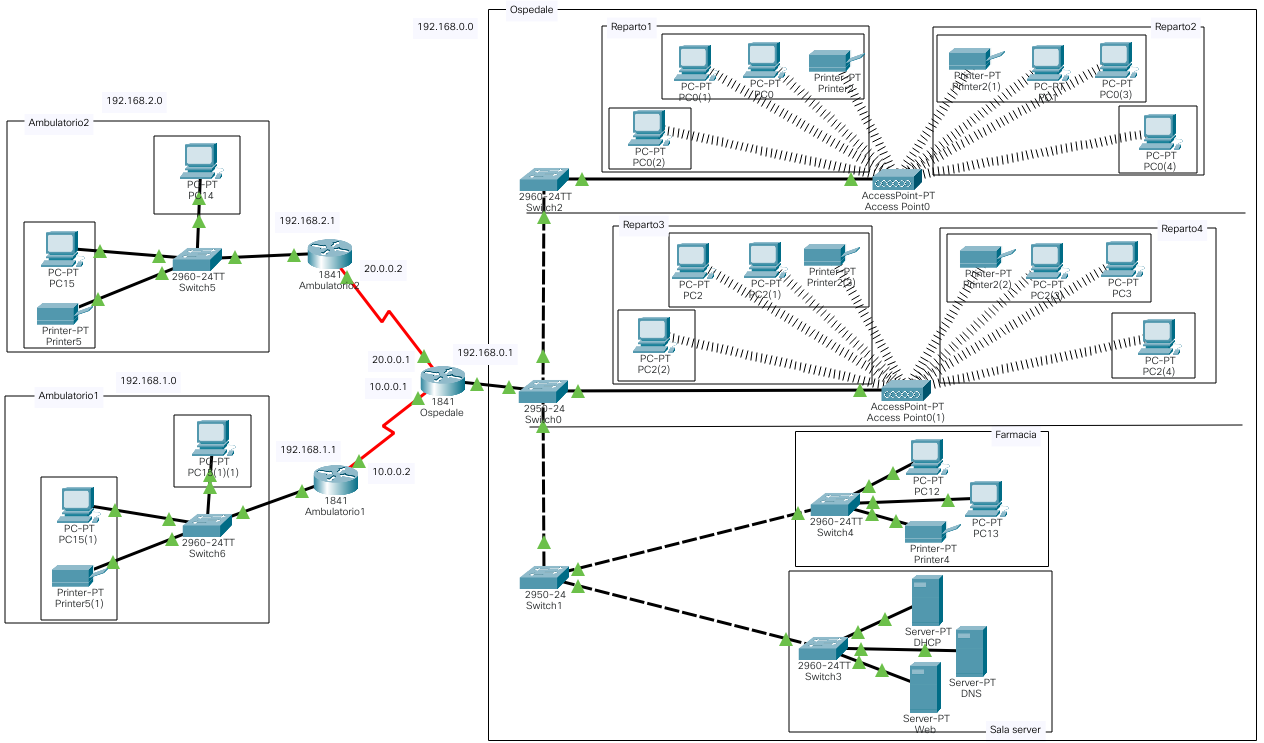
\includegraphics[width=\paperwidth-40pt]{progettazione_rete}}
\end{center}

\section{Configurazione dell'Access Point}
\hspace{24pt}Per questa rete si andrà ad utilizzare un AP con crittografia WEP. L'SSID dell'Access Point del piano terra è 
\mintinline{Batch}{Ospedale2}, mentre quello dell'Access Point del primo piano è \mintinline{Batch}{Ospedale2} e la password 
di accesso è \mintinline{Batch}{3484193820} per entrambi. Il canale utilizzato per la trasmissione del segnale 
(frequenza 2.4GHz) è il 6. Ogni dispositivo che si debba collegare alla WLAN deve scegliere la rete del piano 
ed inserire la password.


\section{Configurazione server web}
\hspace{24pt}L'ospedale ha bisogno di un server web al quale i medici di reparto possono accedere per la gestione dei dati di un 
paziente. Per permettere ciò bisogna abilitare il servizio HTTP\footnote{Hyper-Text Transport Protocol: un protocollo 
per il trasferimento di informazioni tra server e client} sul server incaricato. Dopodiché bisogna assegnare un 
indirizzo IP statico, in questo caso 192.168.0.3. Una volta abilitato il servizio, si caricano i file del sito sul 
server web in modo da renderlo accessibile a tutti gli host collegati alla rete. 

\section{Configurazione DNS}
\hspace{24pt}L'ospedale ha bisogno di un server DNS\footnote{Dynamic Name Service} per l'accesso al server web tramite stringa 
alfanumerica facilmente memorizzabile. Per fare ciò, bisogna abilitare il servizio DNS sul server incaricato ed 
aggiungere un Record contenente nome del sito e l'indirizzo IP del server web, in questo caso rispettivamente 
\mintinline{batch}{portaleinterno.it} e 192.168.0.3. In questo modo tutti gli host connessi alla rete possono accedere 
al server web digitando "portaleinterno.it" sul web browser anziché l'indirizzo ip numerico.

\section{Configurazione DHCP}
\hspace{24pt}È richiesto che a tutti gli host dell'ospedale, esclusi i server, venga assegnato un indirizzo IP tramite 
DHCP. Per fare ciò, bisogna abilitare il servizio DHCP nel server incaricato e impostare l'indirizzo statico del server 
DHCP, l'indirizzo di default gateway, il server DNS, la subnet mask e l'intervallo degli indirizzi da assegnare agli 
host. In questo caso l'indirizzo IP del server sarà 192.168.0.2, l'indirizzo di default gateway è 192.168.0.1, la 
subnet mask è 255.255.255.0 e l'intervallo degli indirizzi da assegnare agli host è .5 $\rightarrow$ .254. L'indirizzo 
di partenza è 192.168.0.5 e il numero massimo di host è 250, escludendo default gateway, broadcast e i server.

\input{test_connettività}

\section{Ipotesi VLAN}
Qualora si voglia permettere l'accesso al router dell'ospedale soltanto alla farmacia bisogna affidarsi alla 
tecnologia VLAN\footnote{Virtual Local Area Network: divisione logica di una rete in più sottoreti agendo sugli 
switch. La topologia fisica della rete non cambia.}. Si andranno a creare delle nuove VLAN all'interno del VLAN 
database degli switch dell'ospedale. \\
\hspace{24pt}Per permettere l'accesso al router soltanto alla farmacia l'unica porta da mettere in modalità 
Access (con soltanto l'id della VLAN della farmacia) è quella del centro stella di edificio collegata al router. 
Tutti i restanti collegamenti saranno impostati su Trunk, in modo da permettere il passaggio di pacchetti provenienti 
da tutte le VLAN.


\vspace*{\fill}
Codice documento LaTeX: \href{https://github.com/Leoooog/EsercitazionePasqua}{Github}

\end{document}



